
%(BEGIN_QUESTION)
% Copyright 2006, Tony R. Kuphaldt, released under the Creative Commons Attribution License (v 1.0)
% This means you may do almost anything with this work of mine, so long as you give me proper credit

An instrumentation student programs a microcontroller to act as a proportional controller, but makes a mistake in writing his program:

$$\includegraphics[width=15.5cm]{i01497x01.eps}$$

\hbox{ \vrule
\vbox{ \hrule \vskip 3pt
\hbox{ \hskip 3pt
\vbox{ \hsize=5in \raggedright

\noindent
\underbar{\bf Pseudocode listing}

{\tt Declare Pin0 as an analog input (scale 0 to 5 volts = 0 to 1023)}

{\tt Declare Pin1 as an analog output (scale 0 to 5 volts = 0 to 1023)}

{\tt Declare SP as a variable, initially set to a value of 614}

{\tt Declare ERROR as a variable}

{\tt Declare GAIN as a variable, initially set to a value of 1.0}

{\tt Declare BIAS as a constant = 614}

{\tt Set ERROR = Pin0 - SP}

\vskip 10pt

{\tt LOOP}

\hskip 10pt {\tt Set Pin1 = (GAIN * ERROR) + BIAS}

{\tt ENDLOOP}

}
\hskip 3pt}%
\vskip 5pt \hrule}%
\vrule}
\vskip 10pt

When executed, this program sets the output to a specific voltage value that never changes as the process variable changes (except when the microcontroller is re-started).  Explain what is wrong with this program, and what is required to fix it.  Also, identify whether this is programmed to be a {\it direct-acting} controller or a {\it reverse-acting} controller.

\underbar{file i01497}
%(END_QUESTION)





%(BEGIN_ANSWER)

This will be a {\it direct-acting} controller, once the programming problem is fixed.

%(END_ANSWER)





%(BEGIN_NOTES)

The {\tt ERROR} calculation is only executed once, before the {\tt LOOP} starts.  This is why the output responds to the process variable only once per re-start of the microcontroller.  To fix this problem, we must move the {\tt ERROR} calculation line inside the {\tt LOOP} where it belongs:

\vskip 10pt

\hbox{ \vrule
\vbox{ \hrule \vskip 3pt
\hbox{ \hskip 3pt
\vbox{ \hsize=5in \raggedright

\noindent
\underbar{\bf Pseudocode listing}

{\tt Declare Pin0 as an analog input (scale 0 to 5 volts = 0 to 1023)}

{\tt Declare Pin1 as an analog output (scale 0 to 5 volts = 0 to 1023)}

{\tt Declare SP as a variable, initially set to a value of 614}

{\tt Declare ERROR as a variable}

{\tt Declare GAIN as a variable, initially set to a value of 1.0}

{\tt Declare BIAS as a constant = 614}

\vskip 10pt

{\tt LOOP}

\hskip 10pt {\tt SET ERROR = Pin0 - SP}

\hskip 10pt {\tt SET Pin1 = (GAIN * ERROR) + BIAS}

{\tt ENDLOOP}

}
\hskip 3pt}%
\vskip 5pt \hrule}%
\vrule}
\vskip 10pt
\vskip 10pt


%INDEX% Control, proportional: digital electronic controller

%(END_NOTES)


